% Options for packages loaded elsewhere
\PassOptionsToPackage{unicode}{hyperref}
\PassOptionsToPackage{hyphens}{url}
%
\documentclass[
]{article}
\usepackage{amsmath,amssymb}
\usepackage{iftex}
\ifPDFTeX
  \usepackage[T1]{fontenc}
  \usepackage[utf8]{inputenc}
  \usepackage{textcomp} % provide euro and other symbols
\else % if luatex or xetex
  \usepackage{unicode-math} % this also loads fontspec
  \defaultfontfeatures{Scale=MatchLowercase}
  \defaultfontfeatures[\rmfamily]{Ligatures=TeX,Scale=1}
\fi
\usepackage{lmodern}
\ifPDFTeX\else
  % xetex/luatex font selection
\fi
% Use upquote if available, for straight quotes in verbatim environments
\IfFileExists{upquote.sty}{\usepackage{upquote}}{}
\IfFileExists{microtype.sty}{% use microtype if available
  \usepackage[]{microtype}
  \UseMicrotypeSet[protrusion]{basicmath} % disable protrusion for tt fonts
}{}
\makeatletter
\@ifundefined{KOMAClassName}{% if non-KOMA class
  \IfFileExists{parskip.sty}{%
    \usepackage{parskip}
  }{% else
    \setlength{\parindent}{0pt}
    \setlength{\parskip}{6pt plus 2pt minus 1pt}}
}{% if KOMA class
  \KOMAoptions{parskip=half}}
\makeatother
\usepackage{xcolor}
\usepackage[margin=1in]{geometry}
\usepackage{color}
\usepackage{fancyvrb}
\newcommand{\VerbBar}{|}
\newcommand{\VERB}{\Verb[commandchars=\\\{\}]}
\DefineVerbatimEnvironment{Highlighting}{Verbatim}{commandchars=\\\{\}}
% Add ',fontsize=\small' for more characters per line
\usepackage{framed}
\definecolor{shadecolor}{RGB}{248,248,248}
\newenvironment{Shaded}{\begin{snugshade}}{\end{snugshade}}
\newcommand{\AlertTok}[1]{\textcolor[rgb]{0.94,0.16,0.16}{#1}}
\newcommand{\AnnotationTok}[1]{\textcolor[rgb]{0.56,0.35,0.01}{\textbf{\textit{#1}}}}
\newcommand{\AttributeTok}[1]{\textcolor[rgb]{0.13,0.29,0.53}{#1}}
\newcommand{\BaseNTok}[1]{\textcolor[rgb]{0.00,0.00,0.81}{#1}}
\newcommand{\BuiltInTok}[1]{#1}
\newcommand{\CharTok}[1]{\textcolor[rgb]{0.31,0.60,0.02}{#1}}
\newcommand{\CommentTok}[1]{\textcolor[rgb]{0.56,0.35,0.01}{\textit{#1}}}
\newcommand{\CommentVarTok}[1]{\textcolor[rgb]{0.56,0.35,0.01}{\textbf{\textit{#1}}}}
\newcommand{\ConstantTok}[1]{\textcolor[rgb]{0.56,0.35,0.01}{#1}}
\newcommand{\ControlFlowTok}[1]{\textcolor[rgb]{0.13,0.29,0.53}{\textbf{#1}}}
\newcommand{\DataTypeTok}[1]{\textcolor[rgb]{0.13,0.29,0.53}{#1}}
\newcommand{\DecValTok}[1]{\textcolor[rgb]{0.00,0.00,0.81}{#1}}
\newcommand{\DocumentationTok}[1]{\textcolor[rgb]{0.56,0.35,0.01}{\textbf{\textit{#1}}}}
\newcommand{\ErrorTok}[1]{\textcolor[rgb]{0.64,0.00,0.00}{\textbf{#1}}}
\newcommand{\ExtensionTok}[1]{#1}
\newcommand{\FloatTok}[1]{\textcolor[rgb]{0.00,0.00,0.81}{#1}}
\newcommand{\FunctionTok}[1]{\textcolor[rgb]{0.13,0.29,0.53}{\textbf{#1}}}
\newcommand{\ImportTok}[1]{#1}
\newcommand{\InformationTok}[1]{\textcolor[rgb]{0.56,0.35,0.01}{\textbf{\textit{#1}}}}
\newcommand{\KeywordTok}[1]{\textcolor[rgb]{0.13,0.29,0.53}{\textbf{#1}}}
\newcommand{\NormalTok}[1]{#1}
\newcommand{\OperatorTok}[1]{\textcolor[rgb]{0.81,0.36,0.00}{\textbf{#1}}}
\newcommand{\OtherTok}[1]{\textcolor[rgb]{0.56,0.35,0.01}{#1}}
\newcommand{\PreprocessorTok}[1]{\textcolor[rgb]{0.56,0.35,0.01}{\textit{#1}}}
\newcommand{\RegionMarkerTok}[1]{#1}
\newcommand{\SpecialCharTok}[1]{\textcolor[rgb]{0.81,0.36,0.00}{\textbf{#1}}}
\newcommand{\SpecialStringTok}[1]{\textcolor[rgb]{0.31,0.60,0.02}{#1}}
\newcommand{\StringTok}[1]{\textcolor[rgb]{0.31,0.60,0.02}{#1}}
\newcommand{\VariableTok}[1]{\textcolor[rgb]{0.00,0.00,0.00}{#1}}
\newcommand{\VerbatimStringTok}[1]{\textcolor[rgb]{0.31,0.60,0.02}{#1}}
\newcommand{\WarningTok}[1]{\textcolor[rgb]{0.56,0.35,0.01}{\textbf{\textit{#1}}}}
\usepackage{graphicx}
\makeatletter
\def\maxwidth{\ifdim\Gin@nat@width>\linewidth\linewidth\else\Gin@nat@width\fi}
\def\maxheight{\ifdim\Gin@nat@height>\textheight\textheight\else\Gin@nat@height\fi}
\makeatother
% Scale images if necessary, so that they will not overflow the page
% margins by default, and it is still possible to overwrite the defaults
% using explicit options in \includegraphics[width, height, ...]{}
\setkeys{Gin}{width=\maxwidth,height=\maxheight,keepaspectratio}
% Set default figure placement to htbp
\makeatletter
\def\fps@figure{htbp}
\makeatother
\setlength{\emergencystretch}{3em} % prevent overfull lines
\providecommand{\tightlist}{%
  \setlength{\itemsep}{0pt}\setlength{\parskip}{0pt}}
\setcounter{secnumdepth}{5}
\usepackage{helvet}
\renewcommand{\familydefault}{\sfdefault}
\usepackage{booktabs}
\usepackage{caption}
\usepackage{longtable}
\ifLuaTeX
  \usepackage{selnolig}  % disable illegal ligatures
\fi
\IfFileExists{bookmark.sty}{\usepackage{bookmark}}{\usepackage{hyperref}}
\IfFileExists{xurl.sty}{\usepackage{xurl}}{} % add URL line breaks if available
\urlstyle{same}
\hypersetup{
  pdftitle={Overview: Study Region and Samples Collected},
  pdfauthor={Sean Kinard},
  hidelinks,
  pdfcreator={LaTeX via pandoc}}

\title{Overview: Study Region and Samples Collected}
\author{Sean Kinard}
\date{2024-06-04}

\begin{document}
\maketitle

{
\setcounter{tocdepth}{2}
\tableofcontents
}
\newpage

\hypertarget{report-summary}{%
\section{Report Summary}\label{report-summary}}

\hypertarget{background}{%
\subsection{Background}\label{background}}

Our investigation encompassed ten coastal rivers and five estuaries,
with a focus on elucidating the connectivity between streams and
estuaries, particularly in the face of aridity and artificial barriers.
The presence of transient taxa (6 amphidromous species, 4 catadromous
species, and 10 euryhaline species) underscored the interconnectedness
of food webs across the coastal prairie landscape.

\hypertarget{approach}{%
\subsection{Approach}\label{approach}}

Through stable isotope analysis of 407 samples, we aimed to decipher
estuarine assimilation in freshwater and transient species, shedding
light on diet composition and source contributions. Relationships
between estuarine assimilation, transient prevalence, annual rainfall,
elevation, dam presence, and distance to the estuary were rigorously
examined. Additionally, the impact of the Calallen Dam on marine
nutrient transport in the Nueces River was assessed.

Analytical scripts are available at:
\url{https://github.com/skkinard/Estimating_Upstream_Nutrient_Subsidies}

\hypertarget{key-features}{%
\subsection{Key Features}\label{key-features}}

This report conducts exploratory data analysis on
\(\delta\)\textsuperscript{13}C and \(\delta\)\textsuperscript{34}S for
monitored streams and the dam study. Notably, the analysis treats
monitored streams separately from the dam study due to variations in
sampling methods---fish and invertebrate sampling at the Nueces River
employed different techniques (seining and kicknets), and there is a
lack of long-term monitoring survey data available for the Nueces River.

The report features scaperplots, illustrating animal mixtures and
sources in a 2-dimensional isotopic space. Additionally, it presents
summary statistics for stable isotope values, offering valuable insights
for fellow researchers.

\hypertarget{relevance}{%
\subsection{Relevance}\label{relevance}}

In ecological stable isotope studies, it is imperative to include
scatterplots in 2-dimensional isotopic space and report summary
statistics for all analyzed values. These visual representations offer
insights into the distribution and relationships between isotopic
values, aiding in the identification of patterns, trends, and potential
outliers within the data. By examining scatterplots, researchers can
discern clusters or patterns indicative of different ecological groups
or sources of isotopic variation, facilitating the interpretation of
trophic relationships, habitat use, and migration patterns within
ecosystems. Additionally, summary statistics provide a quantitative
summary of the central tendency and variability of isotopic values,
allowing researchers to assess data quality, compare between sites or
species, and communicate findings effectively to the scientific
community and stakeholders. Overall, these analytical tools are
essential for understanding ecological processes, ensuring data
reliability, and facilitating knowledge dissemination in ecological
stable isotope research.

\newpage

\hypertarget{satterplot-delta34s-versus-delta13c-streams}{%
\subsubsection{\texorpdfstring{Satterplot
\(\delta\)\textsuperscript{34}S versus \(\delta\)\textsuperscript{13}C:
Streams}{Satterplot \textbackslash delta34S versus \textbackslash delta13C: Streams}}\label{satterplot-delta34s-versus-delta13c-streams}}

\(\delta\)\textsuperscript{34}S versus \(\delta\)\textsuperscript{13}C
values for fish and invertebrates, shaped and colored according to their
migratory habits. Labels mark mean source signatures from streams and
estuaries with cross-hairs extending to the 95\% confidence interval.

\begin{Shaded}
\begin{Highlighting}[]
\FunctionTok{source}\NormalTok{(here}\SpecialCharTok{::}\FunctionTok{here}\NormalTok{(}\StringTok{\textquotesingle{}03\_public\textquotesingle{}}\NormalTok{, }\StringTok{\textquotesingle{}calculation\textquotesingle{}}\NormalTok{, }\StringTok{\textquotesingle{}24\_CS\_mix\_vis\_region.R\textquotesingle{}}\NormalTok{))}

\NormalTok{plot\_scatter\_transient}
\end{Highlighting}
\end{Shaded}

\begin{center}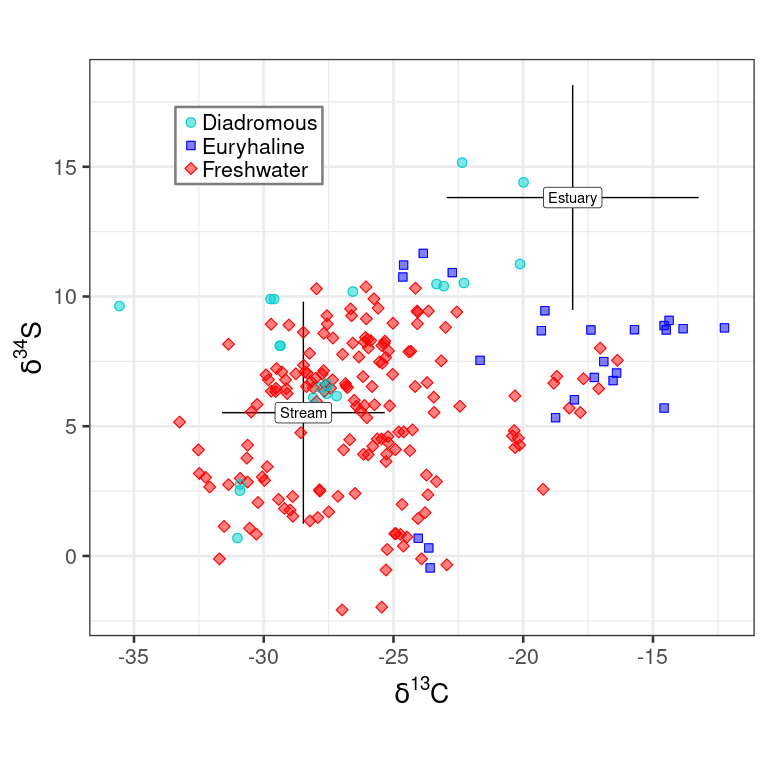
\includegraphics{02_Stable_Isotope_EDA_files/figure-latex/unnamed-chunk-2-1} \end{center}

\newpage

\hypertarget{satterplot-delta34s-versus-delta13c-calallen-dam}{%
\subsubsection{\texorpdfstring{Satterplot
\(\delta\)\textsuperscript{34}S versus \(\delta\)\textsuperscript{13}C:
Calallen
Dam}{Satterplot \textbackslash delta34S versus \textbackslash delta13C: Calallen Dam}}\label{satterplot-delta34s-versus-delta13c-calallen-dam}}

Fish and invertebrate \(\delta\)\textsuperscript{34}S and
\(\delta\)\textsuperscript{13}C signatures above (red) and below (blue)
Calallen Dam on the Nueces River (0-1 m elevation and 20 km from the
nearest Estuary). Labelled cross-hairs mark source signatures and 95\%
confidence intervals from streams and estuaries.

\begin{Shaded}
\begin{Highlighting}[]
\NormalTok{plot\_scatter\_dam}
\end{Highlighting}
\end{Shaded}

\begin{center}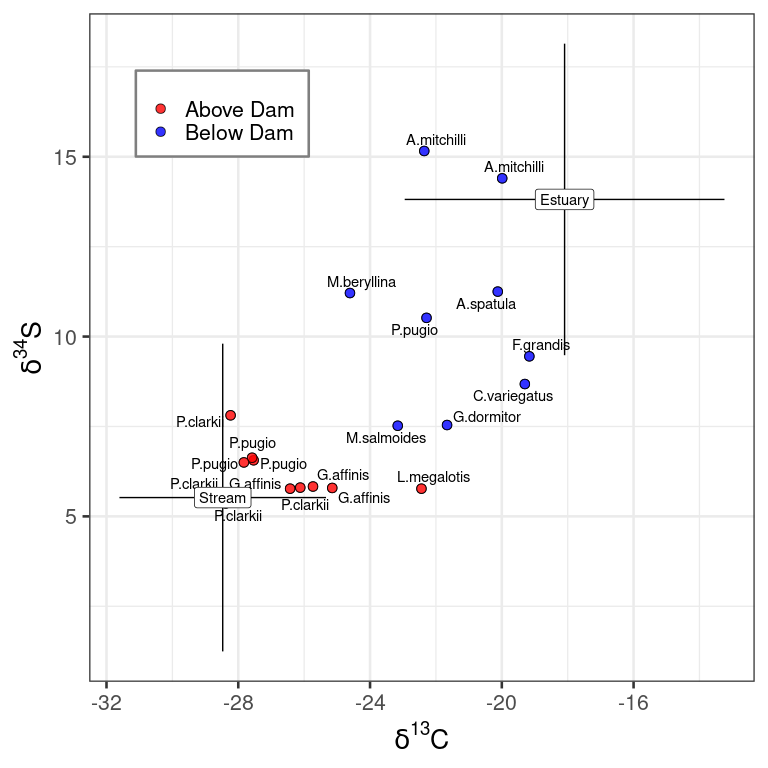
\includegraphics{02_Stable_Isotope_EDA_files/figure-latex/unnamed-chunk-3-1} \end{center}

\newpage

\hypertarget{supplemental-1}{%
\subsubsection{Supplemental 1}\label{supplemental-1}}

Bootstrapped mean and 95\% confidence intervals for primary producer
δ\textsuperscript{13}C and δ\textsuperscript{34}S signatures from
streams and estuaries.

\begin{Shaded}
\begin{Highlighting}[]
\NormalTok{table\_source\_boot }\SpecialCharTok{\%\textgreater{}\%}
  \FunctionTok{mutate}\NormalTok{(}\AttributeTok{isotope =} \FunctionTok{ifelse}\NormalTok{(isotope }\SpecialCharTok{==} \StringTok{\textquotesingle{}carbon\textquotesingle{}}\NormalTok{, }\StringTok{\textquotesingle{}Carbon{-}13\textquotesingle{}}\NormalTok{, }\StringTok{\textquotesingle{}Sulfur{-}34\textquotesingle{}}\NormalTok{)) }\SpecialCharTok{\%\textgreater{}\%}
  \FunctionTok{gt}\NormalTok{() }\SpecialCharTok{\%\textgreater{}\%}
  \FunctionTok{cols\_align}\NormalTok{(}\AttributeTok{align =}\StringTok{\textquotesingle{}center\textquotesingle{}}\NormalTok{) }\SpecialCharTok{\%\textgreater{}\%} 
  \FunctionTok{fmt\_number}\NormalTok{(}\AttributeTok{decimals=}\DecValTok{1}\NormalTok{) }\SpecialCharTok{\%\textgreater{}\%}
  \FunctionTok{cols\_label}\NormalTok{(}
    \AttributeTok{isotope =} \StringTok{"Isotope"}\NormalTok{,}
    \AttributeTok{mu =} \StringTok{"Mean (\textbackslash{}U03B4)"}\NormalTok{,}
    \AttributeTok{lower =} \StringTok{"2.5\% (\textbackslash{}U03B4)"}\NormalTok{,}
    \AttributeTok{upper =} \StringTok{"97.5\% (\textbackslash{}U03B4)"}\NormalTok{,}
    \AttributeTok{.fn =}\NormalTok{ md)}
\end{Highlighting}
\end{Shaded}

\begin{longtable}{cccc}
\toprule
Isotope & Mean (δ) & 2.5\% (δ) & 97.5\% (δ) \\ 
\midrule
\multicolumn{4}{l}{Estuary} \\ 
\midrule
Carbon-13 & $-18.1$ & $-19.7$ & $-16.5$ \\ 
Sulfur-34 & $13.8$ & $12.4$ & $15.2$ \\ 
\midrule
\multicolumn{4}{l}{Stream} \\ 
\midrule
Carbon-13 & $-28.5$ & $-29.2$ & $-27.7$ \\ 
Sulfur-34 & $5.5$ & $4.5$ & $6.5$ \\ 
\bottomrule
\end{longtable}

\newpage

\hypertarget{supplemental-7}{%
\subsubsection{Supplemental 7}\label{supplemental-7}}

Primary producer \(\delta\)\textsuperscript{34}S and
\(\delta\)\textsuperscript{13} summary statistics grouped according to
site and sample type. Cell contents contain ``mean, standard deviation
(n)''.

\begin{Shaded}
\begin{Highlighting}[]
\FunctionTok{setwd}\NormalTok{(}\StringTok{"/home/kinard/Documents/Research/Dissertation/03\_Diadromy"}\NormalTok{)}

\NormalTok{table\_iso\_sources }\SpecialCharTok{\%\textgreater{}\%}
  \FunctionTok{add\_rain}\NormalTok{() }\SpecialCharTok{\%\textgreater{}\%}
  \FunctionTok{mutate}\NormalTok{(}\AttributeTok{annualrain=}\FunctionTok{round}\NormalTok{(annualrain,}\DecValTok{0}\NormalTok{)) }\SpecialCharTok{\%\textgreater{}\%}
  \FunctionTok{arrange}\NormalTok{(site\_type, annualrain, lowest\_taxon) }\SpecialCharTok{\%\textgreater{}\%}
  \FunctionTok{group\_by}\NormalTok{(site\_type, lowest\_taxon) }\SpecialCharTok{\%\textgreater{}\%}
  \FunctionTok{gt}\NormalTok{() }\SpecialCharTok{\%\textgreater{}\%}
  \FunctionTok{cols\_align}\NormalTok{(}\AttributeTok{align =}\StringTok{\textquotesingle{}left\textquotesingle{}}\NormalTok{) }\SpecialCharTok{\%\textgreater{}\%}
  \FunctionTok{fmt\_missing}\NormalTok{(}\AttributeTok{missing\_text =} \StringTok{""}\NormalTok{) }\SpecialCharTok{\%\textgreater{}\%} 
  \FunctionTok{cols\_label}\NormalTok{(}\AttributeTok{site\_code =} \StringTok{"Location"}\NormalTok{,}
             \AttributeTok{annualrain =} \StringTok{\textquotesingle{}Annual Rain (cm)\textquotesingle{}}\NormalTok{,}
             \AttributeTok{C13 =} \StringTok{\textquotesingle{}\textbackslash{}U03B4 Carbon{-}13\textquotesingle{}}\NormalTok{,}
             \AttributeTok{S34 =} \StringTok{"\textbackslash{}U03B4 Sulfur{-}34"}\NormalTok{)}
\end{Highlighting}
\end{Shaded}

\begin{longtable}{llll}
\toprule
Location & Annual Rain (cm) & δ Carbon-13 & δ Sulfur-34 \\ 
\midrule
\multicolumn{4}{l}{Estuary - Algae} \\ 
\midrule
BB &  & -17.5, 3.1 (2) & 17.1, 0.8 (2) \\ 
CB &  & -23.2,     (1) & 19.9,     (1) \\ 
HB &  & -16.7, 4.3 (2) & 18.7, 1.8 (2) \\ 
LB &  & -17.5,     (1) & 17.2,     (1) \\ 
NB &  & -23.6, 0.2 (2) & 19.0, 0.6 (2) \\ 
\midrule
\multicolumn{4}{l}{Estuary - Detritus} \\ 
\midrule
BB &  & -14.5, 0.9 (2) & 7.52, 4.0 (2) \\ 
CB &  & -13.1, 0.2 (2) & 11.0, 2.6 (2) \\ 
HB &  & -17.0, 2.6 (4) & 14.6, 0.6 (4) \\ 
LB &  & -20.5, 7.1 (2) & 9.81, 0.3 (2) \\ 
NB &  & -15.4, 0.8 (2) & 9.68, 4.5 (2) \\ 
\midrule
\multicolumn{4}{l}{Estuary - Macrophyte} \\ 
\midrule
BB &  & -16.1, 5.1 (3) & 16.5, 2.9 (3) \\ 
CB &  & -19.5, 6.4 (4) & 15.2, 2.6 (4) \\ 
HB &  & -13.4,     (1) & 13.6,     (1) \\ 
LB &  & -20.2, 10.1 (2) & 13.9, 5.7 (2) \\ 
NB &  & -21.9, 6.4 (3) & 7.78, 1.9 (3) \\ 
\midrule
\multicolumn{4}{l}{Stream - Algae} \\ 
\midrule
TR & 54 & -18.7,     (1) & 9.06,     (1) \\ 
AR & 69 & -29.0, 0.7 (3) & 2.33, 0.09 (3) \\ 
MR & 73 & -29.7, 2.7 (2) & 11.2, 1.6 (2) \\ 
PD & 79 & -23.4,     (1) & 10.1,     (1) \\ 
PL & 82 & -25.6, 0.2 (2) & 12.5, 0.04 (2) \\ 
GC & 84 & -31.2, 0.3 (2) & 4.66, 0.3 (2) \\ 
\midrule
\multicolumn{4}{l}{Stream - Detritus} \\ 
\midrule
TR & 54 & -29.9, 1.7 (3) & 9.01, 1.1 (3) \\ 
SF & 57 & -26.8, 3.0 (2) & 1.62, 0.007 (2) \\ 
AR & 69 & -27.8, 3.3 (6) & 4.04, 0.7 (6) \\ 
MR & 73 & -27.4, 1.9 (3) & 4.26, 2.9 (3) \\ 
PL & 82 & -28.4, 1.4 (2) & 5.46, 0.5 (2) \\ 
GC & 84 & -29.2, 1.4 (7) & 0.697, 4.0 (7) \\ 
WM & 94 & -27.9, 0.4 (2) & 2.61, 2.3 (2) \\ 
EM & 95 & -29.1, 1.0 (3) & 5.5, 0.9 (3) \\ 
\midrule
\multicolumn{4}{l}{Stream - Periphyton} \\ 
\midrule
TR & 54 & -25.6,     (1) & 11.9,     (1) \\ 
SF & 57 & -15.2,     (1) & 12.9,     (1) \\ 
AR & 69 & -23.0,     (1) & 4.25,     (1) \\ 
MR & 73 & -23.8,     (1) & 14.5,     (1) \\ 
PD & 79 & -27.3,     (1) & 9.1,     (1) \\ 
PL & 82 & -20.5,     (1) & 4.11,     (1) \\ 
GC & 84 & -23.4,     (1) & 11.3,     (1) \\ 
EM & 95 & -21.2, 0.5 (2) & 9.13, 0.3 (2) \\ 
\midrule
\multicolumn{4}{l}{Stream - Riparian Leaves} \\ 
\midrule
TR & 54 & -23.4, 7.3 (4) & 11.8, 1.8 (4) \\ 
PD & 79 & -29.2,     (1) & 16.9,     (1) \\ 
GC & 84 & -30.4, 1.7 (5) & 1.03, 2.0 (5) \\ 
\midrule
\multicolumn{4}{l}{Stream - Macrophyte} \\ 
\midrule
SF & 57 & -30.1,     (1) & -1.54,     (1) \\ 
AR & 69 & -30.3, 1.3 (3) & 3.81, 0.7 (3) \\ 
MR & 73 & -30.2, 1.6 (3) & 9.12, 0.5 (3) \\ 
PD & 79 & -28.7, 1.2 (2) & 9.64, 1.7 (2) \\ 
GC & 84 & -30.4, 1.9 (4) & 4.63, 1.2 (4) \\ 
WM & 94 & -29.2, 2.6 (3) & 7.23, 1.8 (3) \\ 
EM & 95 & -27.9, 0.07 (2) & 8.2, 0.0 (2) \\ 
\bottomrule
\end{longtable}

\newpage

\hypertarget{supplemental-8}{%
\subsubsection{Supplemental 8}\label{supplemental-8}}

Stream fish \(\delta\)\textsuperscript{34}S and
\(\delta\)\textsuperscript{13} summary statistics grouped by taxanomic
family. Cell contents contain ``mean, standard deviation (n)''.

\begin{Shaded}
\begin{Highlighting}[]
\FunctionTok{setwd}\NormalTok{(}\StringTok{"/home/kinard/Documents/Research/Dissertation/03\_Diadromy"}\NormalTok{)}

\NormalTok{table\_iso\_stream }\SpecialCharTok{\%\textgreater{}\%}
  \FunctionTok{filter}\NormalTok{(guild}\SpecialCharTok{==}\StringTok{\textquotesingle{}Fish\textquotesingle{}}\NormalTok{) }\SpecialCharTok{\%\textgreater{}\%}
  \FunctionTok{select}\NormalTok{(}\SpecialCharTok{{-}}\NormalTok{guild, }\SpecialCharTok{{-}}\NormalTok{site\_type) }\SpecialCharTok{\%\textgreater{}\%}
  \FunctionTok{add\_rain}\NormalTok{() }\SpecialCharTok{\%\textgreater{}\%}
  \FunctionTok{mutate}\NormalTok{(}\AttributeTok{annualrain=}\FunctionTok{round}\NormalTok{(annualrain,}\DecValTok{0}\NormalTok{)) }\SpecialCharTok{\%\textgreater{}\%}
  \FunctionTok{arrange}\NormalTok{(family, annualrain) }\SpecialCharTok{\%\textgreater{}\%}
  \FunctionTok{group\_by}\NormalTok{(family) }\SpecialCharTok{\%\textgreater{}\%}
  \FunctionTok{gt}\NormalTok{() }\SpecialCharTok{\%\textgreater{}\%}
  \FunctionTok{cols\_align}\NormalTok{(}\AttributeTok{align =}\StringTok{\textquotesingle{}center\textquotesingle{}}\NormalTok{) }\SpecialCharTok{\%\textgreater{}\%} 
  \FunctionTok{cols\_label}\NormalTok{(}\AttributeTok{site\_code =} \StringTok{"Location"}\NormalTok{,}
             \AttributeTok{annualrain =} \StringTok{\textquotesingle{}Annual Rain (cm)\textquotesingle{}}\NormalTok{,}
             \AttributeTok{C13 =} \StringTok{\textquotesingle{}\textbackslash{}U03B4 Carbon{-}13\textquotesingle{}}\NormalTok{,}
             \AttributeTok{S34 =} \StringTok{"\textbackslash{}U03B4 Sulfur{-}34"}\NormalTok{)}
\end{Highlighting}
\end{Shaded}

\begin{longtable}{cccc}
\toprule
Location & Annual Rain (cm) & δ Carbon-13 & δ Sulfur-34 \\ 
\midrule
\multicolumn{4}{l}{Centrarchidae} \\ 
\midrule
TR & 54 & -18.4, 0.5 (4) & 6.53, 0.6 (4) \\ 
SF & 57 & -21.6, 1.8 (8) & 3.13, 2.5 (8) \\ 
AR & 69 & -25.6, 1.3 (21) & 3.83, 1.3 (21) \\ 
MR & 73 & -30.1, 4.4 (2) & 1.54, 5.1 (2) \\ 
PD & 79 & -25.3, 1.0 (7) & 7.36, 0.8 (7) \\ 
PL & 82 & -23.7, 0.6 (8) & 9.21, 0.7 (8) \\ 
GC & 84 & -30.3, 1.4 (16) & 2.53, 1.1 (16) \\ 
WM & 94 & -27.9, 1.0 (23) & 6.56, 0.6 (23) \\ 
EM & 95 & -26.3, 1.4 (10) & 8.08, 0.7 (10) \\ 
\midrule
\multicolumn{4}{l}{Cichlidae} \\ 
\midrule
TR & 54 & -18.2, 1.5 (2) & 4.51, 2.7 (2) \\ 
SF & 57 & -24.8, 0.8 (4) & 0.368, 2.2 (4) \\ 
AR & 69 & -26.4, 1.3 (3) & 3.46, 0.8 (3) \\ 
MR & 73 & -31.4,     (1) & 8.16,     (1) \\ 
PD & 79 & -27.2, 1.0 (3) & 9.98, 0.6 (3) \\ 
\midrule
\multicolumn{4}{l}{Cyprinodontidae} \\ 
\midrule
TR & 54 & -14.1, 1.3 (5) & 8.81, 0.2 (5) \\ 
\midrule
\multicolumn{4}{l}{Eleotridae} \\ 
\midrule
PL & 82 & -26.6,     (1) & 10.2,     (1) \\ 
\midrule
\multicolumn{4}{l}{Fundulidae} \\ 
\midrule
TR & 54 & -17.2, 0.9 (6) & 7.04, 1.1 (6) \\ 
PD & 79 & -25.8,     (1) & 9.91,     (1) \\ 
\midrule
\multicolumn{4}{l}{Ictaluridae} \\ 
\midrule
AR & 69 & -26.7,     (1) & 4.48,     (1) \\ 
PD & 79 & -27.0, 2.8 (2) & 8.94, 0.05 (2) \\ 
GC & 84 & -30.4, 0.2 (2) & 0.955, 0.2 (2) \\ 
EM & 95 & -25.7, 0.5 (3) & 7.6, 0.1 (3) \\ 
\midrule
\multicolumn{4}{l}{Pecidae} \\ 
\midrule
WM & 94 & -29.6, 0.3 (3) & 7.1, 0.1 (3) \\ 
\midrule
\multicolumn{4}{l}{Poeciliidae} \\ 
\midrule
TR & 54 & -16.9, 2.0 (7) & 6.6, 1.6 (7) \\ 
SF & 57 & -23.7, 0.2 (6) & 1.24, 1.3 (6) \\ 
MR & 73 & -29.7,     (1) & 8.93,     (1) \\ 
PL & 82 & -23.7, 1.0 (3) & 11.1, 0.5 (3) \\ 
GC & 84 & -30.5, 0.2 (4) & 3.56, 1.5 (4) \\ 
WM & 94 & -28.7, 1.4 (3) & 6.22, 0.3 (3) \\ 
\bottomrule
\end{longtable}

\newpage

\hypertarget{supplemental-9}{%
\subsubsection{Supplemental 9}\label{supplemental-9}}

Stream invertebrate \(\delta\)\textsuperscript{34}S and
\(\delta\)\textsuperscript{13} summary statistics grouped by taxanomic
family. Cell contents contain ``mean, standard deviation (n)''.

\begin{Shaded}
\begin{Highlighting}[]
\FunctionTok{setwd}\NormalTok{(}\StringTok{"/home/kinard/Documents/Research/Dissertation/03\_Diadromy"}\NormalTok{)}

\NormalTok{table\_iso\_stream }\SpecialCharTok{\%\textgreater{}\%}
  \FunctionTok{filter}\NormalTok{(guild}\SpecialCharTok{==}\StringTok{\textquotesingle{}Invertebrate\textquotesingle{}}\NormalTok{) }\SpecialCharTok{\%\textgreater{}\%}
  \FunctionTok{select}\NormalTok{(}\SpecialCharTok{{-}}\NormalTok{guild, }\SpecialCharTok{{-}}\NormalTok{site\_type) }\SpecialCharTok{\%\textgreater{}\%}
  \FunctionTok{add\_rain}\NormalTok{() }\SpecialCharTok{\%\textgreater{}\%}
  \FunctionTok{mutate}\NormalTok{(}\AttributeTok{annualrain=}\FunctionTok{round}\NormalTok{(annualrain,}\DecValTok{0}\NormalTok{)) }\SpecialCharTok{\%\textgreater{}\%}
  \FunctionTok{arrange}\NormalTok{(family, annualrain) }\SpecialCharTok{\%\textgreater{}\%}
  \FunctionTok{group\_by}\NormalTok{(family) }\SpecialCharTok{\%\textgreater{}\%}
  \FunctionTok{gt}\NormalTok{() }\SpecialCharTok{\%\textgreater{}\%}
  \FunctionTok{cols\_align}\NormalTok{(}\AttributeTok{align =}\StringTok{\textquotesingle{}center\textquotesingle{}}\NormalTok{) }\SpecialCharTok{\%\textgreater{}\%} 
  \FunctionTok{cols\_label}\NormalTok{(}\AttributeTok{site\_code =} \StringTok{"Location"}\NormalTok{,}
             \AttributeTok{annualrain =} \StringTok{\textquotesingle{}Annual Rain (cm)\textquotesingle{}}\NormalTok{,}
             \AttributeTok{C13 =} \StringTok{\textquotesingle{}\textbackslash{}U03B4 Carbon{-}13\textquotesingle{}}\NormalTok{,}
             \AttributeTok{S34 =} \StringTok{"\textbackslash{}U03B4 Sulfur{-}34"}\NormalTok{)}
\end{Highlighting}
\end{Shaded}

\begin{longtable}{cccc}
\toprule
Location & Annual Rain (cm) & δ Carbon-13 & δ Sulfur-34 \\ 
\midrule
\multicolumn{4}{l}{Aeshnidae} \\ 
\midrule
AR & 69 & -28.6,     (1) & 4.02,     (1) \\ 
\midrule
\multicolumn{4}{l}{Baetidae} \\ 
\midrule
GC & 84 & -35.4,     (1) & 3.71,     (1) \\ 
\midrule
\multicolumn{4}{l}{Belastomatidae} \\ 
\midrule
EM & 95 & -31.3,     (1) & 11.0,     (1) \\ 
\midrule
\multicolumn{4}{l}{Cambaridae} \\ 
\midrule
SF & 57 & -24.8, 0.3 (5) & 0.61, 0.3 (5) \\ 
AR & 69 & -26.0,     (1) & 5.33,     (1) \\ 
PD & 79 & -26.4, 0.5 (3) & 8.38, 0.7 (3) \\ 
PL & 82 & -26.3, 0.6 (3) & 9.44, 0.2 (3) \\ 
GC & 84 & -31.8, 0.4 (2) & 1.9, 1.1 (2) \\ 
WM & 94 & -29.6, 0.1 (3) & 6.38, 0.07 (3) \\ 
EM & 95 & -26.4, 0.8 (3) & 8.35, 0.05 (3) \\ 
\midrule
\multicolumn{4}{l}{Coenagrionidae} \\ 
\midrule
AR & 69 & -26.1,     (1) & 4.41,     (1) \\ 
MR & 73 & -32.7,     (1) & 8.66,     (1) \\ 
GC & 84 & -31.2,     (1) & 1.4,     (1) \\ 
EM & 95 & -31.8,     (1) & 8.59,     (1) \\ 
\midrule
\multicolumn{4}{l}{Corduliidae} \\ 
\midrule
GC & 84 & -31.3,     (1) & -0.57,     (1) \\ 
\midrule
\multicolumn{4}{l}{Gomphidae} \\ 
\midrule
GC & 84 & -29.6,     (1) & 0.11,     (1) \\ 
EM & 95 & -29.0,     (1) & 7.13,     (1) \\ 
\midrule
\multicolumn{4}{l}{Gyrinidae} \\ 
\midrule
MR & 73 & -32.1,     (1) & 8.99,     (1) \\ 
\midrule
\multicolumn{4}{l}{Hyalellidae} \\ 
\midrule
GC & 84 & -33.9,     (1) & 2.13,     (1) \\ 
EM & 95 & -30.9,     (1) & 8.05,     (1) \\ 
\midrule
\multicolumn{4}{l}{Naucoridae} \\ 
\midrule
MR & 73 & -21.8,     (1) & 10.7,     (1) \\ 
\midrule
\multicolumn{4}{l}{Nepidae} \\ 
\midrule
EM & 95 & -21.0,     (1) & 8.8,     (1) \\ 
\midrule
\multicolumn{4}{l}{Palaemonidae} \\ 
\midrule
MR & 73 & -35.6,     (1) & 9.63,     (1) \\ 
PD & 79 & -29.7, 0.09 (2) & 9.9, 0.0 (2) \\ 
PL & 82 & -23.2, 0.2 (2) & 10.4, 0.06 (2) \\ 
GC & 84 & -30.9, 0.06 (3) & 1.99, 1.1 (3) \\ 
WM & 94 & -27.6, 0.5 (3) & 6.17, 0.08 (3) \\ 
EM & 95 & -29.4, 0.02 (2) & 8.1, 0.0 (2) \\ 
\midrule
\multicolumn{4}{l}{Panopeidae} \\ 
\midrule
CB & NA & -18.8,     (1) & 15.7,     (1) \\ 
\midrule
\multicolumn{4}{l}{Physidae} \\ 
\midrule
EM & 95 & -28.9,     (1) & 9.82,     (1) \\ 
\midrule
\multicolumn{4}{l}{Planorbidae} \\ 
\midrule
EM & 95 & -33.5,     (1) & 9.11,     (1) \\ 
\midrule
\multicolumn{4}{l}{Portunidae} \\ 
\midrule
PL & 82 & -25.4,     (1) & 9.95,     (1) \\ 
\midrule
\multicolumn{4}{l}{Thiaridae} \\ 
PD & 79 & -16.2,     (1) & 12.0,     (1) \\ 
\bottomrule
\end{longtable}

\newpage

\hypertarget{supplemental-10}{%
\subsubsection{Supplemental 10}\label{supplemental-10}}

Fish and invertebrates caught above and below Calallen Dam
\(\delta\)\textsuperscript{34}S and \(\delta\)\textsuperscript{13}
summary statistics. Samples were grouped by taxonomic family. Cell
contents contain ``mean, standard deviation (n)''.

\begin{Shaded}
\begin{Highlighting}[]
\NormalTok{table\_iso\_dam }\SpecialCharTok{\%\textgreater{}\%}
  \FunctionTok{mutate}\NormalTok{(}\AttributeTok{site\_code =} \FunctionTok{ifelse}\NormalTok{(site\_code }\SpecialCharTok{==} \StringTok{\textquotesingle{}UN\textquotesingle{}}\NormalTok{, }\StringTok{\textquotesingle{}Above Dam\textquotesingle{}}\NormalTok{, }\StringTok{\textquotesingle{}Below Dam\textquotesingle{}}\NormalTok{)) }\SpecialCharTok{\%\textgreater{}\%}
  \FunctionTok{group\_by}\NormalTok{(site\_type, guild, family) }\SpecialCharTok{\%\textgreater{}\%}
  \FunctionTok{arrange}\NormalTok{(site\_type, family, site\_code) }\SpecialCharTok{\%\textgreater{}\%}
  \FunctionTok{fix\_site\_order}\NormalTok{() }\SpecialCharTok{\%\textgreater{}\%}
  \FunctionTok{gt}\NormalTok{() }\SpecialCharTok{\%\textgreater{}\%}
  \FunctionTok{cols\_align}\NormalTok{(}\AttributeTok{align =}\StringTok{\textquotesingle{}left\textquotesingle{}}\NormalTok{) }\SpecialCharTok{\%\textgreater{}\%} 
    \FunctionTok{cols\_label}\NormalTok{(}\AttributeTok{site\_code =} \StringTok{"Location"}\NormalTok{,}
               \AttributeTok{C13 =} \StringTok{\textquotesingle{}\textbackslash{}U03B4 Carbon{-}13\textquotesingle{}}\NormalTok{,}
               \AttributeTok{S34 =} \StringTok{"\textbackslash{}U03B4 Sulfur{-}34"}\NormalTok{)}
\end{Highlighting}
\end{Shaded}

\begin{longtable}{lll}
\toprule
Location & δ Carbon-13 & δ Sulfur-34 \\ 
\midrule
\multicolumn{3}{l}{Stream - Fish - Atherinopsidae} \\ 
\midrule
Below Dam & -24.6,     (1) & 11.2,     (1) \\ 
\midrule
\multicolumn{3}{l}{Stream - Invertebrate - Belastomatidae} \\ 
\midrule
Above Dam & -27.5,     (1) & 6.92,     (1) \\ 
\midrule
\multicolumn{3}{l}{Stream - Invertebrate - Cambaridae} \\ 
\midrule
Above Dam & -27.8, 1.1 (4) & 6.14, 1.1 (4) \\ 
\midrule
\multicolumn{3}{l}{Stream - Fish - Centrarchidae} \\ 
\midrule
Above Dam & -22.4,     (1) & 5.77,     (1) \\ 
Below Dam & -23.2,     (1) & 7.52,     (1) \\ 
\midrule
\multicolumn{3}{l}{Stream - Invertebrate - Chironomidae} \\ 
\midrule
Below Dam & -25.6,     (1) & 3.45,     (1) \\ 
\midrule
\multicolumn{3}{l}{Stream - Invertebrate - Coenagrionidae} \\ 
\midrule
Above Dam & -29.1, 0.2 (2) & 5.8, 0.2 (2) \\ 
\midrule
\multicolumn{3}{l}{Stream - Fish - Cyprinodontidae} \\ 
\midrule
Below Dam & -19.3,     (1) & 8.68,     (1) \\ 
\midrule
\multicolumn{3}{l}{Stream - Fish - Eleotridae} \\ 
\midrule
Below Dam & -21.7,     (1) & 7.54,     (1) \\ 
\midrule
\multicolumn{3}{l}{Stream - Fish - Engraulidae} \\ 
\midrule
Below Dam & -21.2, 1.7 (2) & 14.8, 0.5 (2) \\ 
\midrule
\multicolumn{3}{l}{Stream - Fish - Fundulidae} \\ 
\midrule
Below Dam & -19.2,     (1) & 9.45,     (1) \\ 
\midrule
\multicolumn{3}{l}{Stream - Invertebrate - Gomphidae} \\ 
\midrule
Above Dam & -26.5,     (1) & 6.18,     (1) \\ 
\midrule
\multicolumn{3}{l}{Stream - Invertebrate - Hyalellidae} \\ 
\midrule
Above Dam & -26.2,     (1) & 5.82,     (1) \\ 
\midrule
\multicolumn{3}{l}{Stream - Fish - Lepisosteidae} \\ 
\midrule
Below Dam & -20.1,     (1) & 11.2,     (1) \\ 
\midrule
\multicolumn{3}{l}{Stream - Invertebrate - Naucoridae} \\ 
\midrule
Above Dam & -26.2,     (1) & 8.17,     (1) \\ 
\midrule
\multicolumn{3}{l}{Stream - Invertebrate - Palaemonidae} \\ 
\midrule
Above Dam & -27.6, 0.2 (3) & 6.56, 0.07 (3) \\ 
Below Dam & -22.3,     (1) & 10.5,     (1) \\ 
\midrule
\multicolumn{3}{l}{Stream - Invertebrate - Panopeidae} \\ 
\midrule
Below Dam & -20.5, 0.4 (3) & 10.3, 1.3 (3) \\ 
\midrule
\multicolumn{3}{l}{Stream - Invertebrate - Physidae} \\ 
\midrule
Above Dam & -26.3,     (1) & 6.11,     (1) \\ 
\midrule
\multicolumn{3}{l}{Stream - Fish - Poeciliidae} \\ 
Above Dam & -25.8, 0.6 (3) & 5.8, 0.03 (3) \\ 
\bottomrule
\end{longtable}

\end{document}
